\documentclass[12pt]{thesul}
%----------------------------------------------------------------------
%                               Packages
%----------------------------------------------------------------------
\usepackage[french]{babel}
\usepackage{acronym} % \ac[p], \acl[p], \acs[p], \acf[p]
\usepackage[maxbibnames=99,maxcitenames=1,sorting=none]{biblatex}
\bibliography{biblio.bib}
\usepackage{booktabs} % \toprule, \midrule, \cmidrule, \bottomrule
\usepackage{cancel} % \cancel
\usepackage{caption}
\usepackage{csquotes}
\usepackage{hyperref}
\hypersetup{hidelinks}
\usepackage[inline]{enumitem}
\setlist[enumerate]{label=(\roman*)} %% <- set the base level label separately
\usepackage{import} % \import
\usepackage[french]{minitoc}

\usepackage{xcolor}
\AtBeginDocument{
\definecolor{lfsgreen}{RGB}{31,160,31}
\definecolor{lfsorange}{RGB}{255,178,2}
\definecolor{lfsred}{RGB}{160,30,31}

% white
\definecolor{uclwhite}{rgb}{1, 1, 1}

%   UCL style guide colours.
%   Number refer to level of tint.
%   100%    1
%    70%    2
%    50%    3
%    20%    4

 % UCL style guide dk purple
\definecolor{ucl1dkpurple}{RGB}{82,66,91}
\definecolor{ucl2dkpurple}{RGB}{134,122,140}
\definecolor{ucl3dkpurple}{RGB}{168,160,173}
\definecolor{ucl4dkpurple}{RGB}{220,217,222}

 % UCL style guide dk red
\definecolor{ucl1dkred}{RGB}{90,27,49}
\definecolor{ucl2dkred}{RGB}{139,95,110}
\definecolor{ucl3dkred}{RGB}{172,141,152}
\definecolor{ucl4dkred}{RGB}{222,209,214}

 % UCL style guide dk blue
\definecolor{ucl1dkblue}{RGB}{0,67,89}
\definecolor{ucl2dkblue}{RGB}{76,123,138}
\definecolor{ucl3dkblue}{RGB}{127,161,172}
\definecolor{ucl4dkblue}{RGB}{204,217,222}

 % UCL style guide dk green
\definecolor{ucl1dkgreen}{RGB}{75,70,32}
\definecolor{ucl2dkgreen}{RGB}{129,125,98}
\definecolor{ucl3dkgreen}{RGB}{165,162,143}
\definecolor{ucl4dkgreen}{RGB}{219,218,210}

 % UCL style guide black
\definecolor{ucl1black}{RGB}{0,0,0}
\definecolor{ucl2black}{RGB}{75,75,75}
\definecolor{ucl3black}{RGB}{128,128,128}
\definecolor{ucl4black}{RGB}{205,205,205}

 % UCL style guide pink
\definecolor{ucl1pink}{RGB}{145,24,83}
\definecolor{ucl2pink}{RGB}{178,93,134}
\definecolor{ucl3pink}{RGB}{200,139,169}
\definecolor{ucl4pink}{RGB}{233,209,221}

 % UCL style guide md red
\definecolor{ucl1mdred}{RGB}{195,58,45}
\definecolor{ucl2mdred}{RGB}{213,117,108}
\definecolor{ucl3mdred}{RGB}{225,156,150}
\definecolor{ucl4mdred}{RGB}{243,216,213}

 % UCL style guide md blue
\definecolor{ucl1mdblue}{RGB}{69,156,189}
\definecolor{ucl2mdblue}{RGB}{124,186,209}
\definecolor{ucl3mdblue}{RGB}{162,205,222}
\definecolor{ucl4mdblue}{RGB}{218,235,242}

 % UCL style guide md green
\definecolor{ucl1mdgreen}{RGB}{130,141,55}
\definecolor{ucl2mdgreen}{RGB}{167,175,115}
\definecolor{ucl3mdgreen}{RGB}{192,198,155}
\definecolor{ucl4mdgreen}{RGB}{230,232,215}

 % UCL style guide orange
\definecolor{ucl1orange}{RGB}{215,123,35}
\definecolor{ucl2orange}{RGB}{227,162,101}
\definecolor{ucl3orange}{RGB}{235,189,145}
\definecolor{ucl4orange}{RGB}{247,229,211}

  % UCL style guide lt purple
\definecolor{ucl1ltpurple}{RGB}{191,175,188}
\definecolor{ucl2ltpurple}{RGB}{210,199,208}
\definecolor{ucl3ltpurple}{RGB}{223,215,221}
\definecolor{ucl4ltpurple}{RGB}{242,239,242}

 % UCL style guide yellow
\definecolor{ucl1yellow}{RGB}{229,175,0}
\definecolor{ucl2yellow}{RGB}{237,199,76}
\definecolor{ucl3yellow}{RGB}{242,215,127}
\definecolor{ucl4yellow}{RGB}{250,239,204}

 % UCL style guide lt blue
\definecolor{ucl1ltblue}{RGB}{168,192,209}
\definecolor{ucl2ltblue}{RGB}{194,211,223}
\definecolor{ucl3ltblue}{RGB}{211,223,232}
\definecolor{ucl4ltblue}{RGB}{238,242,246}

% UCL style guide brt green
\definecolor{ucl1brtgreen}{RGB}{204,209,88}
\definecolor{ucl2brtgreen}{RGB}{219,223,138}
\definecolor{ucl3brtgreen}{RGB}{229,232,171}
\definecolor{ucl4brtgreen}{RGB}{245,246,222}

% UCL style guide stone
\definecolor{ucl1stone}{RGB}{217,214,204}
\definecolor{ucl2stone}{RGB}{228,226,219}
\definecolor{ucl3stone}{RGB}{236,234,229}
\definecolor{ucl4stone}{RGB}{255,255,255}

% UCL style guide lt green
\definecolor{ucl1ltgreen}{RGB}{185,193,147}
\definecolor{ucl2ltgreen}{RGB}{206,211,179}
\definecolor{ucl3ltgreen}{RGB}{220,224,201}
\definecolor{ucl4ltgreen}{RGB}{241,243,233}

\definecolor{darkgreen}{RGB}{75,70,32}
\definecolor{darkblue}{RGB}{0,67,89}
\definecolor{mydarkblue}{RGB}{76,123,138}
\definecolor{mydarkblueid}{RGB}{0,67,89}
\definecolor{mylightblue}{RGB}{168,192,209}
\definecolor{mydarkorange}{RGB}{215,123,35}
\definecolor{mylightorange}{RGB}{227,162,101}
\definecolor{mydarkred}{RGB}{90,27,49}
\definecolor{mydarkpurple}{RGB}{134,122,140}
\definecolor{mydarkpurpleid}{RGB}{82,66,91}
}

\usepackage{amssymb}
\usepackage{amsmath}
\usepackage{amsthm}
% \interdisplaylinepenalty=2500
\theoremstyle{definition}
\newtheorem{definition}{Définition}
\newtheorem{subdefinition}{Définition}[definition]
\newtheorem{myrule}{Règle}
\newtheorem{property}{Propriété}
\newtheorem{subproperty}{Propriété}[property]
\usepackage{MnSymbol} % \dashrightarrow

\usepackage{algorithm, algpseudocode}
\floatname{algorithm}{Algorithme} % Renomme caption de "Algorithm" -> "Algorithme"

\newcommand\CONDITION[2]%
  {\begin{tabular}[t]{@{}l@{}l@{}}
     #1&#2
   \end{tabular}%
  }
  \algdef{SE}[WHILE]{While}{EndWhile}[1]%
  {\algorithmicwhile\ \CONDITION{#1}{\ \algorithmicdo}}%
  {\algorithmicend\ \algorithmicwhile}
\algdef{SE}[FOR]{For}{EndFor}[1]%
  {\algorithmicfor\ \CONDITION{#1}{\ \algorithmicdo}}%
  {\algorithmicend\ \algorithmicfor}
\algdef{S}[FOR]{ForAll}[1]%
  {\algorithmicforall\ \CONDITION{#1}{\ \algorithmicdo}}
\algdef{SE}[REPEAT]{Repeat}{Until}{\algorithmicrepeat}[1]%
  {\algorithmicuntil\ \CONDITION{#1}{}}
\algdef{SE}[IF]{If}{EndIf}[1]%
  {\algorithmicif\ \CONDITION{#1}{\ \algorithmicthen}}%
  {\algorithmicend\ \algorithmicif}%
\algdef{C}[IF]{IF}{ElsIf}[1]%
  {\algorithmicelse\ \algorithmicif\ \CONDITION{#1}{\ \algorithmicthen}}

\usepackage[inline,nomargin,index]{fixme}
\fxsetup{theme=color,mode=multiuser,inlineface=\itshape,envface=\itshape}
\FXRegisterAuthor{mn}{amn}{Matthieu}

\usepackage{tikz} % \begin{tikzpicture} \end{tikzpicture}
\usetikzlibrary{calc}
\usetikzlibrary{graphs}
\usetikzlibrary{quotes}
\usetikzlibrary{shapes.misc}

\usepackage[caption=false,font=footnotesize,labelfont=sf,textfont=sf]{subfig}

\usepackage{marvosym} % \Flatsteel
\usepackage{wasysym} % \checked

\usepackage{pifont} % \ding
\renewcommand{\checkmark}{\ding{51}}
\newcommand{\ballotx}{\ding{55}}

\usepackage{xspace} % \xspace

% Commands
%---------
\newcommand{\cf}[1]{(cf. \autoref{#1}, page \pageref{#1})}
\newcommand{\eg}{e.g.\xspace}
\newcommand{\ie}{c.-à-d.\xspace}

\newcommand{\hb}{\emph{happens-before}\xspace}

\newcommand{\inbb}[1]{\in \mathbb{#1}}
\newcommand{\new}{\textbf{new}}
\newcommand{\trm}[1]{\mathit{#1}}
\newcommand{\set}[1]{\left\{#1\right\}} % set brace notation

\newcommand{\betterid}[3]{\trm{#1}^{\trm{#2}}_{\trm{#3}}}
\newcommand{\id}[3]{$\trm{#1}^{\trm{#2}}_{\trm{#3}}$}
\newcommand{\epoch}[1]{$\varepsilon_{#1}$}
\newcommand{\lid}{<_{id}}
\newcommand{\leqid}{$\leq_{id}$~}
\newcommand{\lepoch}{$<_{\varepsilon}$~}
\newcommand{\leqepoch}{$\leq_{\varepsilon}$~}
\newcommand{\ltuple}{<_{t}}

\newcommand{\botn}{\bot_\mathbb{N}}
\newcommand{\topn}{\top_\mathbb{N}}
\newcommand{\logootuple}[1]{\langle \text{pos}_{#1},\text{nodeId}_{#1},\text{seq}_{#1} \rangle}

\newcommand{\bigO}[1]{$\mathcal{O}(#1)$}

\newcommand{\widthletter}{2em}
\newcommand{\widthblock}{3em}
\newcommand{\widthoriginepoch}{1.33em}
\newcommand{\widthepoch}{1.65em}

\newcommand{\withmathbreak}[1]{\parbox{\linewidth}{#1}}
\newcommand{\elt}{E}
\newcommand{\nat}{\mathbb{N}}


% Définit noms pour \autoref
%---------
\newcommand{\algorithmautorefname}{Algorithme}
\newcommand{\annexautorefname}{Annexe}
\newcommand{\definitionautorefname}{Définition}
\newcommand{\propertyautorefname}{Propriété}
\newcommand{\subfigureautorefname}{Figure}
\newcommand{\subpropertyautorefname}{Propriété}

% Tikz styles
\tikzset{
    common/.style={anchor=west, draw, rectangle, minimum height=6mm},
    letter/.style={common, minimum width=\widthletter},
    block/.style={common, minimum width=\widthblock},
    epoch/.style={letter, rounded rectangle, rounded rectangle east arc=0pt, minimum width=\widthepoch},
    point/.style={insert path={ node[scale=5*sqrt(\pgflinewidth)]{.} }},
    node/.style={draw, circle, minimum size=1em},
    op/.style={draw, circle, minimum size=2.7em},
    causalop/.style={op, double=white, inner sep=2pt},
    gc-rule-1/.style={dashed, thick, darkblue},
    gc-rule-2/.style={densely dotted, thick, darkgreen},
    cross/.style={
        path picture={
            \draw[ucl1dkred, very thick]
                (path picture bounding box.south east)--(path picture bounding box.north west)
                (path picture bounding box.south west)--(path picture bounding box.north east);
        }
    }
}


%-------------------------------------------------------------------
%                             Marges
%-------------------------------------------------------------------

% pour positionner les vraies marges:
%\SetRealMargins{1mm}{1mm}

%-------------------------------------------------------------------
%                             En-têtes
%-------------------------------------------------------------------

% Les en-têtes: quelques exemples
%\UppercaseHeadings
%\UnderlineHeadings
%\newcommand\bfheadings[1]{{\bf #1}}
%\FormatHeadingsWith{\bfheadings}
%\FormatHeadingsWith{\uppercase}
%\FormatHeadingsWith{\underline}
\newcommand\upun[1]{\uppercase{\underline{\underline{#1}}}}
\FormatHeadingsWith\upun

\newcommand\itheadings[1]{\textit{#1}}
\FormatHeadingsWith{\itheadings}

% pour avoir un trait sous l'en-tete:
\setlength{\HeadRuleWidth}{0.4pt}

%-------------------------------------------------------------------
%                         Les références
%-------------------------------------------------------------------

\NoChapterNumberInRef
\NoChapterPrefix

%-------------------------------------------------------------------
%                           Brouillons
%-------------------------------------------------------------------

% ceci ajoute une marque « brouillon » et la date
\ThesisDraft

%-------------------------------------------------------------------
%                   Pour collecter un glossaire et un index
%-------------------------------------------------------------------

\makeglossary
\makeindex

%-------------------------------------------------------------------
%                           Acronymes
%-------------------------------------------------------------------

% Acronyms
% --------
% \input{assets/acronyms.tex}
\acrodef{ADT}[ADT]{Abstract Data Type}
\acrodefplural{ADT}[ADTs]{Abstract Data Types}
\acrodef{API}[API]{Application Programming Interface}
\acrodef{AW}[AW]{\emph{Add-Wins}}
\acrodef{CCI}[CCI]{Convergence, Causality preservation, Intention preservation}
\acrodef{CL}[CL]{\emph{Causal-Length}}
\acrodef{CRDT}[CRDT]{Conflict-free Replicated Data Type}
\acrodefplural{CRDT}[CRDTs]{Conflict-free Replicated Data Types}
\acrodef{DAG}[DAG]{Directed Acyclic Graph}
\acrodef{FIFO}[FIFO]{First In, First Out}
\acrodef{GC}[GC]{Garbage Collection}
\acrodef{IPFS}[IPFS]{InterPlanetary File System}
\acrodef{JIT}[JIT]{Just-In-Time}
\acrodef{LCA}[PPAC]{Plus Petit Ancêtre Commun}
\acrodef{LFS}[LFS]{Local-First Software}
\acrodefplural{LFS}[LFS]{Local-First Softwares}
\acrodef{LUB}[LUB]{Least Upper Bound}
\acrodef{LWW}[LWW]{\emph{Last-Writer-Wins}}
\acrodef{MUTE}[MUTE]{Multi User Text Editor}
\acrodef{MV}[MV]{\emph{Multi-Value}}
\acrodef{OC}[OC]{Commutativité des Opérations}
\acrodef{OT}[OT]{Operational Transformation}
\acrodefplural{OT}[OT]{Operational Transformations}
\acrodef{P2P}[P2P]{Pair-à-Pair}
\acrodef{PKI}[PKI]{Public Key Infrastructure}
\acrodef{PoC}[PoC]{Proof of Concept}
\acrodef{PT}[PT]{Transitivité de la Précédence}
\acrodef{RADT}[RADT]{Replicated Abstract Data Type}
\acrodefplural{RADT}[RADTs]{Replicated Abstract Data Types}
\acrodef{RCB}[RCB]{Reliable Causal Broadcast}
\acrodef{RGA}[RGA]{Replicated Growable Array}
\acrodef{RW}[RW]{\emph{Remove-Wins}}
\acrodef{SEC}[SEC]{Cohérence forte à terme}
\acrodef{TTF}[TTF]{Tombstone Transformation Function}
\acrodefplural{TTF}[TTF]{Tombstone Transformation Functions}
\acrodef{WebRTC}[WebRTC]{Web Real-Time Communication}

%-------------------------------------------------------------------
%                           Couleurs
%-------------------------------------------------------------------

% \input{assets/colours.tex}

%-------------------------------------------------------------------
%                     Global custom tikz commands
%-------------------------------------------------------------------

% \input{assets/tikz_presets.tex}

\begin{document}


      \OddHead={{\leftmark\rightmark}{\hfil\slshape\rightmark}}
      \EvenHead={{\leftmark}{{\slshape\leftmark}\hfil}}
      \OddFoot={\hfil\thepage}
      \EvenFoot={\thepage\hfil}
      \pagestyle{ThesisHeadingsII}


%-------------------------------------------------------------------
%                          Encadrements
%-------------------------------------------------------------------

% encadre les chapitres dans la table des matières:
% (ces commandes doivent figurer apres \begin{document}

\FrameChaptersInToc
%\FramePartsInToc


%-------------------------------------------------------------------
%            Réinitialisation de la numérotation des chapitres
%-------------------------------------------------------------------

% Si la commande suivante est présente,
% elle doit figurer APRÈS \begin{document}
% et avant la première commande \part
\ResetChaptersAtParts

%-------------------------------------------------------------------
%               mini-tables des matières par chapitre
%-------------------------------------------------------------------

% préparer les mini-tables des matières par chapitre.
% (commande de minitoc.sty)
\dominitoc

%-------------------------------------------------------------------
%                         Page de titre:
%-------------------------------------------------------------------

\ThesisTitle{Ré-identification sans coordination dans les types de données répliquées sans conflits (CRDTs)}
\ThesisDate{TODO: Définir une date}
\ThesisAuthor{Matthieu Nicolas}

% Type de la these
\ThesisUL
% Jury:

% (ne pas mettre de \\ apres la dernière entree)

% Exemple de création d'une nouvelle catégorie dans le jury:

% \NewJuryCategory{Encadrants}{\it Encadrant :}
%                        {\it Encadrants :}

\def\blanc{\hspace*{1cm}}

\President    = {À déterminer}
\Rapporteurs  = {Hanifa Boucheneb & Professeure, Polytechnique Montréal\\
                 Davide Frey      & Chargé de recherche, HdR, Inria Rennes Bretagne-Atlantique}
\Examinateurs = {Hala Skaf-Molli  & Maîtresse de conférences, HdR, Nantes Université \\
                 Stephan Merz     & Directeur de Recherche, Inria Nancy - Grand Est}
\Encadrants= {Olivier Perrin      & Professeur des Universités, Université de Lorraine, LORIA \\
              Gérald Oster        & Maître de conférences, Université de Lorraine, LORIA}

%\Invites=       {}

% Création de la page de titre:
\MakeThesisTitlePage

%-------------------------------------------------------------------


%-------------------------------------------------------------------
%                          remerciements
%-------------------------------------------------------------------

%\DontFrameThisInToc
\begin{ThesisAcknowledgments}
WIP
\end{ThesisAcknowledgments}

%-------------------------------------------------------------------
%                            dédicace
%-------------------------------------------------------------------

\begin{ThesisDedication}
WIP
\end{ThesisDedication}


%-------------------------------------------------------------------
%                  écriture de `Chapitre' et `Partie'
%                      dans la table des matières
%-------------------------------------------------------------------

\WritePartLabelInToc
\WriteChapterLabelInToc

%-------------------------------------------------------------------
%                        table des matières
%-------------------------------------------------------------------

\tableofcontents

%-------------------------------------------------------------------
%              Exemple d'utilisation de \SpecialSection
%-------------------------------------------------------------------
%\SpecialSection{Introduction générale}

\DontWriteThisInToc
\listoffigures

\mainmatter
\NumberThisInToc
\chapter{Introduction}
\minitoc

\section{Contexte}
\label{sec:intro-contexte}

L'évolution des technologies du web a conduit à l'avènement de ce qui est communément appelé le Web 2.0.
La principale caractéristique de ce média est la possibilité aux utilisateur-rices non plus seulement de le consulter, mais aussi d'y contribuer.

Ces nouvelles fonctionnalités ont permis l'apparition d'applications incitant les utilisateur-rices à créer et partager leur propre contenu, ainsi que d'échanger avec d'autres utilisateur-rices à ce sujet.
Un cas particulier de ces applications proposent aux utilisateur-rices de travailler ensemble pour la création d'un même contenu, en d'autres termes de collaborer.
Nous appelons ces applications des \emph{systèmes collaboratifs} :
\begin{definition}[Système collaboratif]
  \label{def:collaborative-system}
  Un système collaboratif est un système supportant ses utilisateur-rices dans leurs processus de collaboration pour la réalisation de tâches.
\end{definition}

De nos jours, ces systèmes font parties des applications les plus populaires du paysage internet, \eg GoogleDocs compte XX millions utilisateur-rices, GitHub YY millions, Wikipedia 788 millions {\cite{2022-09-monthly-active-users-wikipedia}} ou Quora 300 millions \cite{2022-01-monthly-active-users-social-networks}.
\mnnote{TODO: Ajouter chiffres et refs}
De leur côté, d'autres plateformes impliquent leur communautés en organisant ponctuellement des collaborations éphémères et généralement massives, \eg r/Place \cite{2022-rplace} ou TwitchPlaysPokemon \cite{2014-twitch-plays-pokemon}.\\

En raison de leur popularité, les systèmes collaboratifs doivent assurer plusieurs propriétés pour garantir leur bon fonctionnement et qualité de service : une haute disponibilité, tolérance aux pannes et capacité de passage à l'échelle.
\begin{definition}[Disponibilité]
  \label{def:availability}
  La disponibilité d'un système indique sa capacité à répondre à tout moment à une requête d'un-e utilisateur-rice.
\end{definition}
\begin{definition}[Tolérance aux pannes]
  La tolérance aux pannes d'un système indique sa capacité à continuer à répondre aux requêtes malgré l'absence de réponse d'un ou plusieurs de ses composants.
\end{definition}
\begin{definition}[Capacité de passage à l'échelle]
  La capacité de passage à l'échelle d'un système indique sa capacité à traiter un volume toujours plus conséquent de requêtes.
\end{definition}

Pour cela, ces systèmes adoptent une architecture décentralisée, que nous illustrons par la \autoref{fig:decentralised-system}.
\begin{figure}[!ht]
  \centering
  \resizebox{0.3 \columnwidth}{!}{
    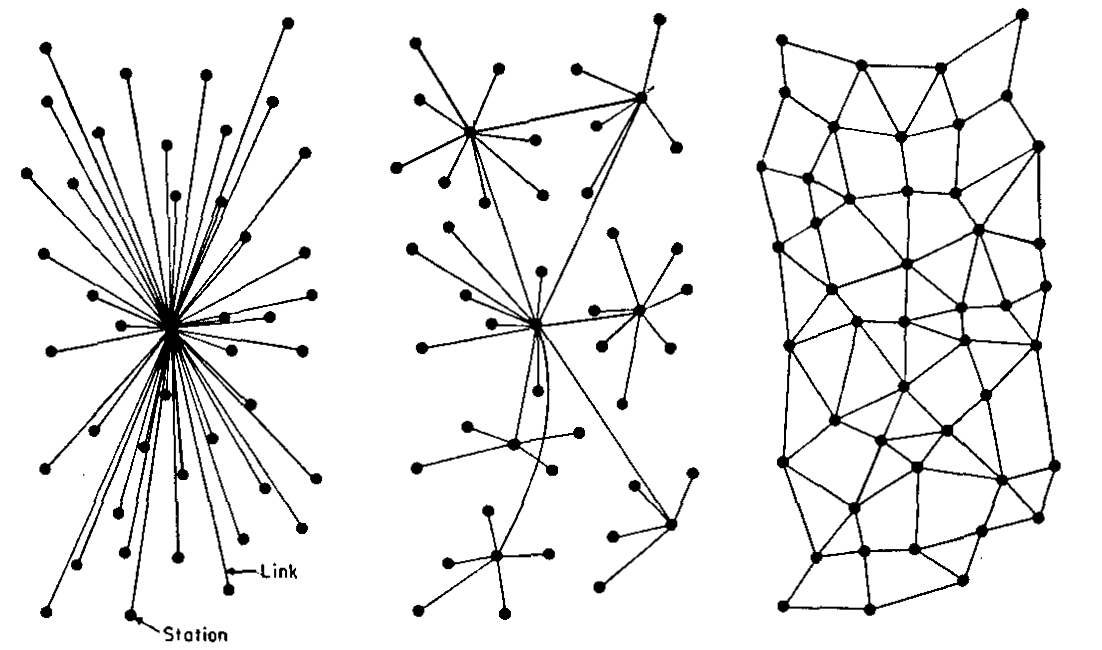
\includegraphics[trim=12cm 0cm 13cm 0cm, clip]{img/centralised-decentralised-distributed}
  }
  \caption[Caption for decentralised-system]{Représentation d'une architecture décentralisée\footnotemark}
  \label{fig:decentralised-system}
\end{figure}
\footnotetext{Source : \cite{1964-distributed-communications-networks-baran}}

Dans ce type d'architecture, les responsabilités, tâches et la charge travail sont réparties entre un ensemble de serveurs.
Il convient toutefois de noter que les serveurs jouent de manière globale toujours un rôle central dans ces systèmes, malgré ce que le nom de cette architecture peut suggérer.
En effet, ces systèmes reposent toujours sur leurs serveurs pour authentifier les utilisateur-rices, stocker les données de leurs utilisateur-rices ou encore fusionner les modifications effectuées par ces dernier-es.\\
% La nuance porte seulement sur le fait que ce n'est plus un serveur unique qui est en charge de ces tâches, mais un ensemble de serveurs.

Bien que cette architecture système permette de répondre aux problèmes d'ordre technique que nous présentons précédemment, nous considérons que cette architecture souffre néanmoins de limites.
Notamment, de part le rôle prédominant que jouent les serveurs dans les systèmes décentralisés, ces derniers échouent à assurer un second ensemble de propriétés, que nous jugeons néanmoins fondamentales :
\begin{definition}[Confidentialité des données]
  \label{def:confidentialite}
  La confidentialité des données d'un système indique sa capacité à garantir à ses utilisateur-rices que leurs données ne seront pas accessibles par des tiers non autorisés ou par le système lui-même.
\end{definition}
\begin{definition}[Souveraineté des données]
  \label{def:souverainete}
  La souveraineté des données d'un système indique sa capacité à garantir à ses utilisateur-rices leur maîtrise de leurs données, \ie leur capacité à les consulter, modifier, partager, exporter; supprimer ou encore à décider de l'usage qui en est fait.
\end{definition}
\begin{definition}[Pérennité]
  \label{def:perennite}
  La pérennité d'un système indique sa capacité à garantir à ses utilisateur-rices son fonctionnement continu dans le temps.
\end{definition}
\begin{definition}[Résistance à la censure]
  \label{def:censorship}
  La résistance à la censure d'un système indique sa capacité à garantir à ses utilisateur-rices son fonctionnement malgré des actions de contrôle de l'information par des autorités.
\end{definition}

De plus, les serveurs ne sont pas une ressource libre.
En effet, ils sont déployés et maintenus par la ou les organisations qui proposent le système collaboratif.
Ces organisations font alors office d'\emph{autorités centrales} du système, \eg en se portant garantes de l'identité des utilisateur-rices, de l'authenticité d'un contenu ou encore de la disponibilité dudit contenu.

De part le fait que les autorités centrales possèdent les serveurs hébergeant le système, elles ont tout pouvoir sur ces derniers.
Ainsi, les utilisateur-rices de systèmes collaboratifs prennent, de manière consciente ou non, le risque que les propriétés présentées précédemment soient transgressées par les autorités auxquelles appartiennent ces applications ou par des tiers avec lesquelles ces autorités interagissent, \eg des gouvernements.
Plusieurs faits d'actualités nous ont malheureusement montré de tels faits, \eg la censure de Wikipedia par des gouvernements \cite{2022-wikipedia-censorship}, la fermeture de services par les entreprises les proposant \cite{2022-killed-by-google} ou encore la mise à disposition des données hébergées par les GAFAMs aux services de renseignement de différentes nations \cite{prism-guardian,prism-washington-post}.
Cependant, le coût de l'infrastructure nécessaire pour déployer des systèmes à large échelle équivalents entrave l'apparition d'alternatives, plus respectueuses de leurs utilisateur-rices.\\

\emph{Ainsi, il nous paraît fondamental de proposer des moyens technologiques rendant accessible la conception et le déploiement des systèmes collaboratifs alternatifs.
Ces derniers devraient minimiser le rôle des autorités centrales, voire l'éliminer, de façon à protéger les intérêts de leurs utilisateur-rices.}\\

Dans cette optique, une piste de recherche que nous jugeons intéressante à étudier est celle des systèmes collaboratifs \acf{P2P}.
Cette architecture système, que nous illustrons par la \autoref{fig:distributed-system}, place les utilisateur-rices au centre du système et relègue les éventuels serveurs à un simple rôle de support de la collaboration, \eg la mise en relation des pairs.

\begin{figure}[!ht]
  \centering
  \resizebox{0.25 \columnwidth}{!}{
    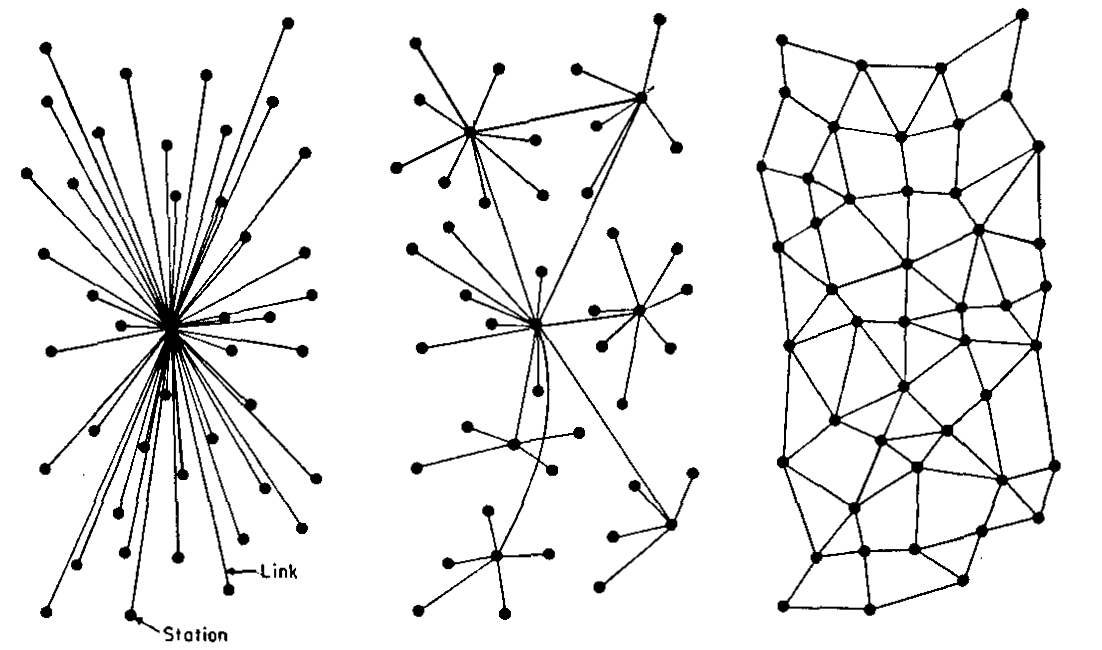
\includegraphics[trim=26cm 0cm 1cm 0cm, clip]{img/centralised-decentralised-distributed}
  }
  \caption[Caption for distributed-system]{Représentation d'une architecture distribuée\footnotemark[\value{footnote}]}
  \label{fig:distributed-system}
\end{figure}

Récemment, la conception de systèmes collaboratifs \ac{P2P} a gagné en traction suite à \cite{localfirstsoftware2019}.
Dans cet article, les auteurs définissent un ensemble de propriétés qui correspondent à celles que nous avons établies précédemment, de la \autoref{def:collaborative-system} à la \autoref{def:censorship}.

En utilisant ces propriétés comme critères, les auteurs comparent les fonctionnalités et garanties offertes par les différents types d'applications, notamment les applications lourdes et les applications basées sur le cloud.

Le résultat de cette comparaison est le suivant : alors que les applications basées sur le cloud permettent de nouveaux usages, notamment la collaboration entre utilisateur-rices ou la synchronisation automatique entre appareils, elles retirent à leurs utilisateur-rices toute garantie de pérennité, confidentialité des données et souveraineté des données.
Ces dernières propriétés sont pourtant communément offertes par les applications lourdes.
La \autoref{fig:lfs-comparison-apps} détaille ce résultat.

\begin{figure}[!ht]
  \centering
  \resizebox{\columnwidth}{!}{
    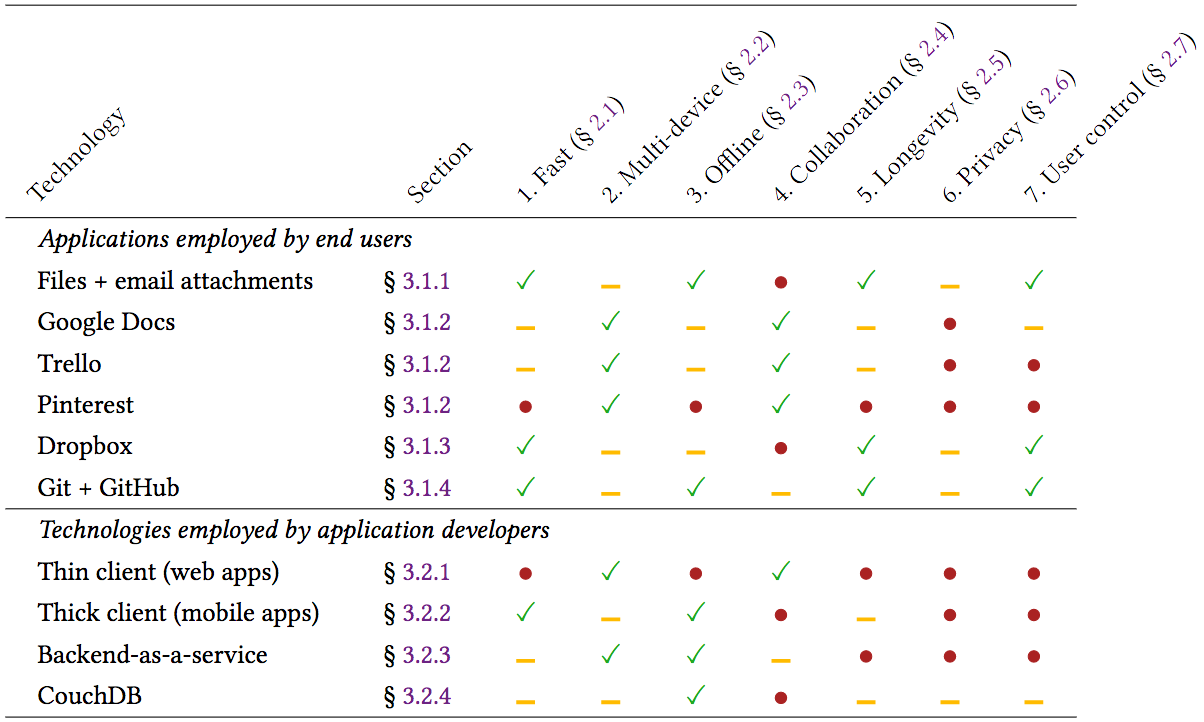
\includegraphics{img/lfs-comparison-apps}
  }
  \caption[Caption for lfs-comparison-apps]{Évaluation d'applications et de technologies vis-à-vis des 7 propriétés visées par les \acl{LFS}\footnotemark}
  \label{fig:lfs-comparison-apps}
\end{figure}

Malgré ce que ce résultat pourrait suggérer, les auteurs affirment que les fonctionnalités de collaboration entre utilisateur-rices ou même de synchronisation entre appareils ne sont pas antinomiques avec les propriétés de confidentialité, souveraineté, pérennité.

Ainsi, ils proposent un nouveau paradigme de conception d'applications collaboratives \ac{P2P}, nommées \acp{LFS}.
Ce paradigme vise à la conception d'applications offrant le meilleur des approches existantes, \ie cochant l'intégralité des critères de la \autoref{fig:lfs-comparison-apps}.
Nous partageons cette vision.\\
% Ce type d'applications se démarque de ceux existants, \eg les applications basées sur le cloud, par la place centrale donnée aux utilisateur-rices et leurs propres appareils, les éventuels serveurs étant relegués qu'à de simples rôles de support.

Cependant, de nombreuses problématiques de recherche identifiées dans \cite{localfirstsoftware2019} sont encore non résolues et entravent la démocratisation des applications \acp{LFS}.
Notamment, les applications \acp{LFS} se doivent de répliquer les données entre appareils pour permettre :
\begin{enumerate}
  \item Le fonctionnement en mode hors-ligne et le fonctionnement avec une faible latence.
  \item Le partage de contenu entre appareils d'un-e même utilisateur-rice.
  \item Le partage de contenu entre utilisateur-rices pour la collaboration.
\end{enumerate}

Toutefois, compte tenu des propriétés visées par les applications \acp{LFS}, plusieurs contraintes restreignent le choix des méthodes de réplication possibles.
Ainsi, pour permettre le fonctionnement en mode hors-ligne de l'application, \ie la consultation et la modification de contenu, les applications \acp{LFS} doivent relaxer la propriété de cohérence des données.
\begin{definition}[Cohérence]
  La cohérence d'un système indique sa capacité à présenter une vue uniforme de son état à chacun de ses utilisateur-rices à un moment donné.
\end{definition}

Les applications \acp{LFS} doivent donc adopter des méthodes de réplication dites optimistes \cite{2005-optimistic-replication-saito}.
Ces méthodes autorisent chaque noeud possédant une copie de la donnée de la consulter et de la modifier sans coordination au préalable avec les autres noeuds\footnote{Par opposition aux méthodes de réplication dites pessimistes, qui nécessitent une coordination préalable entre les noeuds avant toute modification de la donnée.}.
L'état des copies des noeuds peut donc diverger temporairement.
Un mécanisme de synchronisation permet ensuite aux noeuds de partager les modifications effectuées et de les intégrer de façon à converger à terme \cite{10.1145/224057.224070}, \ie obtenir à terme de nouveau des états équivalents.

Cependant, il convient de noter que les méthodes de réplication optimistes autorisent la génération en concurrence de modifications provoquant un conflit, \eg la modification et la suppression d'une même page dans un wiki.
Un mécanisme de résolution de conflits est alors nécessaire pour assurer la convergence à terme des noeuds.

De nouveau, le modèle du système des applications \acp{LFS} limitent les choix possibles concernant les mécanismes de résolution de conflits.
Notamment, les applications \acp{LFS} ne disposent d'aucun contrôle sur le nombre de noeuds qui compose le système, \ie le nombre d'appareils utilisés par l'ensemble de leurs utilisateur-rices.
\mnnote{TODO: Rattacher à la notion d'échelle des réseaux sociaux.}
Le nombre de noeuds peut donc croître de manière non-bornée.
La complexité algorithmique des mécanismes de résolution de conflits doit donc être indépendante de ce paramètre, ou alors en être fonction uniquement de manière logarithmique.

De plus, ces noeuds n'offrent aucune garantie sur leur stabilité.
Des noeuds peuvent donc rejoindre et participer au système, mais uniquement de manière éphèmère.
Ce phénonème est connu sous le nom de \emph{churn} \cite{understandingChurnP2PNetworks2006}.
Ainsi, de part l'absence de garantie sur le nombre de noeuds connectés de manière stable, les applications \acp{LFS} ne peuvent pas utiliser des mécanismes de résolution de conflits reposant sur une coordination synchrone d'une proportion des noeuds du système, \ie sur des algorithmes de consensus \cite{1998-paxos-lamport, 2014-raft-ongaro}.

Ainsi, pour permettre la conception d'applications \acp{LFS}, il convient de disposer de mécanismes de résolution de conflits pour l'ensemble des types de données avec une complexité algorithmique efficace par rapport au nombre de noeuds et ne nécessitant pas de coordination synchrone entre une proportion des noeuds du système.

% \subsection{Réplication de données mutables}

% Les techniques de réplication de données mutables introduisent de la redondance de données dans les systèmes.
% Cette redondance a pour but et effet d'améliorer plusieurs propriétés des systèmes :

% \begin{definition}[Disponibilité]
% \end{definition}

% \begin{definition}[Tolérance aux pannes]
% \end{definition}

% \begin{definition}[Capacité de passage à l'échelle]
% \end{definition}

% \begin{definition}[Latence]
% \end{definition}

% Les techniques de réplication de données peuvent être classées en deux approches : les \emph{techniques de réplication de données pessimistes} et les \emph{techniques de réplication de données optimistes}.
% Ces deux catégories offrent des compromis différents vis-à-vis des propriétés décrites par les théorèmes CAP \cite{brewer_2000_podc} et PACELC \cite{pacelc2012}.
% Notamment, la différence entre ces catégories concerne le cas de la propriété de \emph{cohérence}.

% \begin{definition}[Cohérence]
% \end{definition}

% \subsection{Réplication de données pessimiste}

% Les techniques de réplication de données dites \emph{pessimistes} privilègie la cohérence des données.
% Notamment, ces techniques empêchent les modifications en concurrence d'une même donnée.
% Pour cela, plusieurs approches sont possibles.

% \begin{itemize}
%     \item Première approche consiste à utiliser un verrou.
%     \item Seconde approche consiste à utiliser un système de vote pour décider de la prochaine modification.
%         Consensus, élection de leader, SMR.
%     \item Le choix de privilégier la cohérence des données se fait au détriment de la disponibilité, tolérance aux pannes, capacité de passage à l'échelle et latence.
%         Par exemple, un système basé sur un leader deviendra temporairement indisponible lors d'une panne de son leader, le temps que la panne soit détectée et qu'un nouveau leader soit élu.
% \end{itemize}

% \subsection{Réplication de données optimiste}

% À l'inverse, les techniques de réplication de données dites \emph{optimistes} jugent acceptable de relâcher les contraintes existantes sur la cohérence des données.
% Dans ce paradigme, chaque noeud qui possède une copie de la donnée répliquée peut la consulter et la modifier à tout moment, sans coordination préalable avec les autres noeuds.
% Les copies des noeuds sont donc autorisées à diverger de manière temporaire.

% Les modifications effectuées par chacun sont ensuite diffusées pour être intégrées par l'ensemble des noeuds et converger de nouveau, \ie atteindre des états équivalents.
% Cependant, certaines modifications effectuées en concurrence par les noeuds peuvent provoquer des conflits.
% \mnnote{NOTE: Pourrait insérer exemple de conflits de l'édition collaborative ici.}
% Des mécanismes de résolution de conflits, potentiellement automatiques, sont alors requis pour assurer la convergence à terme.

% Cette approche permet donc de privilégier la disponibilité, tolérance aux pannes, capacité de passage à l'échelle et latence en échange de la cohérence forte.

% Dans le cadre de cette thèse, nous nous intéressons aux techniques de réplication de données optimistes.


\section{Questions de recherche et contributions}
\subsection{Ré-identification sans coordination synchrone pour les \acp{CRDT} pour le type Séquence}
\label{sec:research-questions-rls}

Les \acfp{CRDT}\footnote{\acf{CRDT} : Type de données répliquées sans conflits} \cite{2007-crdt-shapiro,shapiro_2011_crdt} sont des nouvelles spécifications des types de données usuels, \eg l'Ensemble ou la Séquence.
Ils sont conçus pour permettre à un ensemble de noeuds d'un système de répliquer une donnée et pour leur permettre de la consulter, de la modifier sans aucune coordination préalable et d'assurer à terme la convergence des copies.
Dans ce but, les \acp{CRDT} incorporent des mécanismes de résolution de conflits automatiques directement au sein leur spécification.

Cependant, ces mécanimes induisent un surcoût, aussi bien en termes de métadonnées et de calculs que de bande-passante.
Ces surcoûts sont néanmoins jugés acceptables par la communauté pour une variété de types de données, \eg le Registre ou l'Ensemble.
Cependant, le surcoût des \acp{CRDT} pour le type Séquence constitue toujours une problématique de recherche.

En effet, la particularité des \acp{CRDT} pour le type Séquence est que leur surcoût croît de manière monotone au cours de la durée de vie de la donnée, \ie au fur et à mesure des modifications effectuées.
Le surcoût introduit par les \acp{CRDT} pour ce type de données se révèle donc handicapant dans le contexte de collaborations sur de longues durées ou à large échelle.

De manière plus précise, le surcoût des \acp{CRDT} pour le type Séquence provient de la croissance des métadonnées utilisées par leur mécanisme de résolution de conflits automatique.
Ces métadonnées correspondent à des identifiants qui sont associés aux éléments de la Séquence.
Ces identifiants permettent d'intégrer les modifications, \eg en précisant quel est l'élément à supprimer ou en spécifiant la position d'un nouvel élément à insérer par rapport aux autres.

Plusieurs approches ont été proposées pour réduire le coût induit par ces identifiants.
Notamment, \cite{letia:hal-01248270,zawirski:hal-01248197} proposent un mécanisme de ré-assignation des identifiants pour réduire leur coût a posteriori.
Ce mécanisme génère toutefois des conflits en cas de modifications concurrentes de la séquence, \ie l'insertion ou la suppression d'un élément.
Les auteurs résolvent ce problème en proposant un mécanisme de transformation des modifications concurrentes par rapport à l'effet du mécanisme de ré-assignation des identifiants.

Cependant, l'exécution en concurrence du mécanisme de ré-assignation des identifiants par plusieurs noeuds provoque elle-même un conflit.
Pour éviter ce dernier type de conflit, les auteurs choisissent de subordonner à un algorithme de consensus l'exécution du mécanisme de ré-assignation des identifiants.
Ainsi, le mécanisme de ré-assignation des identifiants ne peut être déclenché en concurrence par plusieurs noeuds du système.

Comme nous l'avons évoqué précédemment, reposer sur un algorithme de consensus qui requiert une coordination synchrone entre une proportion de noeuds du système est une contrainte incompatible avec les systèmes \ac{P2P} à large échelle sujets au churn.\\

Notre problématique de recherche est donc la suivante : \emph{pouvons-nous proposer un mécanisme sans coordination synchrone de réduction du surcoût des \acp{CRDT} pour le type Séquence, \ie adapté aux applications \ac{LFS} ?}\\

Pour répondre à cette problématique, nous proposons dans cette thèse RenamableLogootSplit, un nouveau \ac{CRDT} pour le type Séquence.
Ce \ac{CRDT} intègre un mécanisme de ré-assignation des identifiants, dit de renommage, directement au sein de sa spécification.
Nous associons au mécanisme de renommage un mécanisme de résolution de conflits automatique additionnel pour gérer ses exécutions concurrentes.
Finalement, nous définissons un mécanisme de \acf{GC}\footnote{\acf{GC} : Récupération de la mémoire} des métadonnées du mécanisme de renommage pour supprimer à terme son propre surcoût.
De cette manière, nous proposons un \ac{CRDT} pour le type Séquence dont le surcoût est périodiquement réduit, tout en n'introduisant aucune contrainte de coordination synchrone entre les noeuds du système.

\subsection{Éditeur de texte collaboratif \ac{P2P} temps réel chiffré de bout en bout}
\label{sec:research-questions-mute}

Comme évoqué précédemment, la conception d'applications \ac{LFS} à large échelle présente un ensemble de problématiques issues de domaines variés, \eg
\begin{enumerate}
    \item Comment permettre aux utilisateur-rices de collaborer en l'absence d'autorités centrales pour résoudre les conflits de modifications ?
    \item Comment authentifier les utilisateur-rices en l'absence d'autorités centrales ?
    \item Comment structurer le réseau de manière efficace, \ie en limitant le nombre de connexions par pair ?
\end{enumerate}

Cet ensemble de questions peut être résumé en la problématique suivante : \emph{pouvons-nous concevoir une application \ac{LFS} à large échelle, sûre et sans autorités centrales ?}\\

Pour étudier cette problématique, l'équipe Coast développe l'application \acf{MUTE}\footnote{Disponible à l'adresse : \url{https://mutehost.loria.fr}} \cite{MUTE2017}.
Il s'agit d'un \acf{PoC}\footnote{\acf{PoC} : Preuve de concept} d'éditeur de texte web collaboratif \ac{P2P} temps réel chiffré de bout en bout.
Ce projet permet à l'équipe de présenter ses travaux de recherche portant sur les mécanismes de résolutions de conflits automatiques pour le type Séquence \cite{2013-logootsplit,2021-these-vic,2022-rls-tpds-nicolas} et les mécanismes d'authentification des pairs dans les systèmes sans autorités centrales \cite{2018-trusternity-short,2018-trusternity-long}.

De plus, en inscrivant ses travaux dans le cadre d'un système complet, ce projet permet à l'équipe d'identifier de nouvelles problématiques en relation avec les nombreux domaines de recherche nécessaires à la conception d'un tel système, \eg le domaine des protocoles d'appartenance aux groupes \cite{swim2002, lifeguard2018}, des topologies réseaux \ac{P2P} \cite{2018-spray-nedelec} ou encore des protocoles d'établissement de clés de chiffrement de groupe \cite{1995-burmester-desmedt}.\\

Dans le cadre de cette thèse, nous avons contribué au développement de ce projet.
Nous avons notamment implémenté plusieurs \acp{CRDT} pour le type Séquence \cite{2013-logootsplit,2022-rls-tpds-nicolas} et le protocole d'appartenance au réseau SWIM \cite{swim2002}.


\section{Plan du manuscrit}
\begin{itemize}
    \item Ce manuscrit de thèse est organisé de la manière suivante :
    \item Dans le \autoref{chap:state-of-art}, nous introduisons le modèle du système que nous considérons, \ie les systèmes \ac{P2P} à large échelle sujet au churn.
        Puis nous présentons dans ce chapitre l'état de l'art des mécanismes de résolution de conflits automatiques utilisés dans les systèmes adoptant le paradigme de la réplication optimiste.
        À partir de cet état de l'art, nous identifions et motivons notre problématique de recherche, \ie l'absence de mécanisme adapté aux systèmes \ac{P2P} à large échelle sujet au churn permettant de réduire le surcoût induit par les mécanismes de résolution de conflits automatiques pour le type Séquence.
    \item Dans le \autoref{chap:renamablelogootsplit}, nous présentons notre approche pour présenter un tel mécanisme, \ie un mécanisme de résolution de conflits automatiques pour le type Séquence auquel nous associons un mécanisme de \ac{GC} de son surcoût ne nécessitant pas de coordination synchrone entre les noeuds du système.
        Nous détaillons le fonctionnement de notre approche, sa validation par le biais d'une évaluation empirique puis comparons notre approche par rapport aux approches existantes
        Finalement, nous concluons la présentation de notre approche en identifiant et en détaillant plusieurs de ses limites.
    \item Dans le \autoref{chap:mute}, nous présentons \ac{MUTE}, l'éditeur de texte collaboratif temps réel \ac{P2P} chiffré de bout en bout que notre équipe de recherche développe dans le cadre de ses travaux de recherche.
        Nous présentons les différentes couches logicielles formant un pair et les services tiers avec lesquels les pairs interagissent, et détaillons nos travaux dans le cadre de ce projet, \ie l'intégration de notre mécanisme de résolution de conflits automatiques pour le type Séquence et le développement de la couche de livraison des messages associée.
        Pour chaque couche logicielle, nous identifions ses limites et présentons de potentielles pistes d'améliorations.
    \item Finalement, nous récapitulons dans le \autoref{chap:conclusions-perspectives} les contributions réalisées dans le cadre de cette thèse.
        Puis nous clotûrons ce manuscrit en introduisant plusieurs des pistes de recherches que nous souhaiterons explorer dans le cadre de nos travaux futurs.
\end{itemize}


\section{Publications}
Notre travail sur la problématique identifiée dans la \autoref{sec:research-questions-rls}, \ie la proposition d'un mécanisme ne nécessitant aucune coordination synchrone pour réduire le surcoût des \acp{CRDT} pour le type Séquence, a donné lieu à des publications à différents stades de son avancement :
\begin{enumerate}
    \item Dans \cite{2018-rls-middleware-nicolas}, nous motivons le problème identifié et présentons l'idée de notre approche pour y répondre.
    \item Dans \cite{2020-rls-papoc-nicolas}, nous détaillons une première partie de notre approche et présentons notre protocole d'évaluation expérimentale ainsi que ses premiers résultats.
    \item Dans \cite{2022-rls-tpds-nicolas}, nous détaillons notre proposition dans son entièreté.
        Nous accompagnons cette proposition d'une évaluation expérimentale poussée.
        Finalement, nous complétons notre travail d'une discussion analysant ses limites connues et présentant des pistes de travail possibles pour y répondre.
\end{enumerate}
Nous précisons ci-dessous les informations relatives à chacun de ces articles.

\subsection*{Efficient renaming in CRDTs \cite{2018-rls-middleware-nicolas}}

\paragraph{Auteur} Matthieu Nicolas

\paragraph{Article de position} à Middleware 2018 - 19th ACM/IFIP International Middleware Conference (Doctoral Symposium), Dec 2018, Rennes, France.

\paragraph{Abstract}
\emph{Sequence Conflict-free Replicated Data Types (CRDTs)} allow to replicate and edit, without any kind of coordination, sequences in distributed systems.
To ensure convergence, existing works from the literature add metadata to each element but they do not bound its footprint, which impedes their adoption.
Several approaches were proposed to address this issue but they do not fit a fully distributed setting.
In this paper, we present our ongoing work on the design and validation of a fully distributed renaming mechanism, setting a bound to the metadata's footprint.
Addressing this issue opens new perspectives of adoption of these CRDTs in distributed applications.

\subsection*{Efficient Renaming in Sequence CRDTs \cite{2020-rls-papoc-nicolas}}

\paragraph{Auteurs} Matthieu Nicolas, Gérald Oster, Olivier Perrin

\paragraph{Article de workshop} à PaPoC 2020 - 7th Workshop on Principles and Practice of Consistency for Distributed Data, Apr 2020, Heraklion / Virtual, Greece.

\paragraph{Abstract}
To achieve high availability, large-scale distributed systems have to replicate data and to minimise coordination between nodes.
Literature and industry increasingly adopt \acfp{CRDT} to design such systems.
\acp{CRDT} are data types which behave as traditional ones, e.g. the Set or the Sequence.
However, unlike traditional data types, they are designed to natively support concurrent modifications.
To this end, they embed in their specification a conflict-resolution mechanism.

To resolve conflicts in a deterministic manner, \acp{CRDT} usually attach identifiers to elements stored in the data structure.
Identifiers have to comply with several constraints, such as uniqueness or belonging to a dense order.
These constraints may hinder the identifiers’ size from being bounded.
As the system progresses, identifiers tend to grow.
This inflation deepens the overhead of the \ac{CRDT} over time, leading to performance issues.

To address this issue, we propose a new CRDT for Sequence which embeds a renaming mechanism.
It enables nodes to reassign shorter identifiers to elements in an uncoordinated manner.
Experimental results demonstrate that this mechanism decreases the overhead of the replicated data structure and eventually limits it.

\subsection*{Efficient Renaming in Sequence CRDTs \cite{2022-rls-tpds-nicolas}}

\paragraph{Auteurs} Matthieu Nicolas, Gérald Oster, Olivier Perrin

\paragraph{Article de journal} dans IEEE Transactions on Parallel and Distributed Systems, Institute of Electrical and Electronics Engineers, 2022, 33 (12), pp.3870-3885.

\paragraph{Abstract}
To achieve high availability, large-scale distributed systems have to replicate data and to minimise coordination between nodes.
For these purposes, literature and industry increasingly adopt \acfp{CRDT} to design such systems.
\acp{CRDT} are new specifications of existing data types, e.g. Set or Sequence.
While \acp{CRDT} have the same behaviour as previous specifications in sequential executions, they actually shine in distributed settings as they natively support concurrent updates.
To this end, \acp{CRDT} embed in their specification conflict resolution mechanisms.
These mechanisms usually rely on identifiers attached to elements of the data structure to resolve conflicts in a deterministic and coordination-free manner.
Identifiers have to comply with several constraints, such as being unique or belonging to a dense total order.
These constraints may hinder the identifier size from being bounded.
Identifiers hence tend to grow as the system progresses, which increases the overhead of \acp{CRDT} over time and leads to performance issues.
To address this issue, we propose a novel Sequence \ac{CRDT} which embeds a renaming mechanism.
It enables nodes to reassign shorter identifiers to elements in an uncoordinated manner.
Experimental results demonstrate that this mechanism decreases the overhead of the replicated data structure and eventually minimises it.


\import{chapters/etat-art/}{etat-art}
% \import{chapters/rls/}{rls}
% \import{chapters/mute/}{mute}
\import{chapters/conclusion/}{conclusion}
\import{chapters/annexes/}{annexes}

%
%%-------------------------------------------------------------------
%%                         Le glossaire
%%-------------------------------------------------------------------
%\BeginGloWith{Voici un glossaire tout-à-fait fictif,
%              introduit par un texte sur toute la largeur
%              des deux colonnes.}
%\twocolumn
%\PrintGlossary

%-------------------------------------------------------------------
%              L'index (toujours sur deux colonnes)
%-------------------------------------------------------------------
\BeginIndWith{Voici un index}
\PrintIndex

\onecolumn

%-------------------------------------------------------------------
%                       La bibliographie
%-------------------------------------------------------------------

% La bibliographie (comme d'habitude)

%\nocite{*}
%\bibliographystyle{named}

\printbibliography

%-------------------------------------------------------------------
%                          Les résumés
%-------------------------------------------------------------------
% (si le résumé apparaît sur une colonne étroite, avec la
% bibliographie à gauche, c'est sans doute parce que vous avez
% oublié de générer les fichiers d'index et de glossaire...)

\NumberAbstractPages
\begin{ThesisAbstract}
  \begin{FrenchAbstract}
    Afin d'assurer leur haute disponibilité, les systèmes distribués à large échelle se doivent de répliquer leurs données tout en minimisant les coordinations nécessaires entre noeuds.
    Pour concevoir de tels systèmes, la littérature et l'industrie adoptent de plus en plus l'utilisation de types de données répliquées sans conflits (CRDTs).
    Les CRDTs sont des types de données qui offrent des comportements similaires aux types existants, tel l'Ensemble ou la Séquence.
    Ils se distinguent cependant des types traditionnels par leur spécification, qui supporte nativement les modifications concurrentes.
    À cette fin, les CRDTs incorporent un mécanisme de résolution de conflits au sein de leur spécification.

    Afin de résoudre les conflits de manière déterministe, les CRDTs associent généralement des identifiants aux éléments stockés au sein de la structure de données.
    Les identifiants doivent respecter un ensemble de contraintes en fonction du CRDT, telles que l'unicité ou l'appartenance à un ordre dense.
    Ces contraintes empêchent de borner la taille des identifiants.
    La taille des identifiants utilisés croît alors continuellement avec le nombre de modifications effectuées, aggravant le surcoût lié à l'utilisation des CRDTs par rapport aux structures de données traditionnelles.
    Le but de cette thèse est de proposer des solutions pour pallier ce problème.

    Nous présentons dans cette thèse deux contributions visant à répondre à ce problème :
    \begin{enumerate*}
      \item Un nouveau CRDT pour Séquence, RenamableLogootSplit, qui intègre un mécanisme de renommage à sa spécification.
      Ce mécanisme de renommage permet aux noeuds du système de réattribuer des identifiants de taille minimale aux éléments de la séquence.
      Cependant, cette première version requiert une coordination entre les noeuds pour effectuer un renommage.
      L'évaluation expérimentale montre que le mécanisme de renommage permet de réinitialiser à chaque renommage le surcoût lié à l'utilisation du CRDT.
      \item Une seconde version de RenamableLogootSplit conçue pour une utilisation dans un système distribué.
      Cette nouvelle version permet aux noeuds de déclencher un renommage sans coordination préalable.
      L'évaluation expérimentale montre que cette nouvelle version présente un surcoût temporaire en cas de renommages concurrents, mais que ce surcoût est à terme.
    \end{enumerate*}
    \KeyWords{CRDTs, édition collaborative en temps réel, cohérence à terme, optimisation mémoire, performance}
  \end{FrenchAbstract}
  \begin{EnglishAbstract}
    \KeyWords{CRDTs, real-time collaborative editing, eventual consistency, memory-wise optimisation, performance}
  \end{EnglishAbstract}
\end{ThesisAbstract}


\end{document}



